\documentclass[../DoAn.tex]{subfiles}
\begin{document}
Chương này trình bày chi tiết về thiết kế phần mềm của hệ thống giám sát GNSS tích hợp. Mục tiêu của thiết kế là đảm bảo hệ thống hoạt động ổn định, hiệu quả và có khả năng thích ứng với môi trường hoạt động của các thiết bị IoT. Nội dung chương bao gồm kiến trúc tổng thể của phần mềm, mô hình phân lớp chức năng, mô tả chi tiết từng mô-đun chính và cơ chế tương tác giữa chúng. Ngoài ra, chương cũng tập trung vào các giải pháp tối ưu hiệu suất xử lý và tiết kiệm năng lượng, nhằm nâng cao độ tin cậy và kéo dài thời gian vận hành của thiết bị trong điều kiện thực tế. Các sơ đồ và bảng minh họa được sử dụng để hỗ trợ việc diễn giải kiến trúc và luồng dữ liệu trong hệ thống.
\section{Kiến trúc tổng thể hệ thống}
\label{section:4.1}
Hệ thống được xây dựng với mục tiêu giám sát vị trí thiết bị di động một cách tiết kiệm năng lượng và hiệu quả. Kiến trúc tổng thể bao gồm hai thành phần chính: một thiết bị vi điều khiển ATmega8 và một thiết bị Android tích hợp module GNSS. Hai thành phần này hoạt động phối hợp để đảm bảo việc thu thập và truyền dữ liệu chỉ diễn ra khi thực sự cần thiết.

Vi điều khiển ATmega8 có nhiệm vụ giám sát cảm biến rung. Khi phát hiện rung, ATmega8 sẽ kích hoạt mô-đun GNSS và thiết bị Android thông qua chân điều khiển nguồn (PWRKEY). Ngược lại, nếu không còn phát hiện chuyển động trong một khoảng thời gian xác định, vi điều khiển sẽ chủ động tắt nguồn thiết bị Android nhằm tiết kiệm năng lượng cho toàn hệ thống.

Thiết bị Android sau khi được bật sẽ thực hiện các chức năng thu thập dữ liệu GNSS, kiểm tra tọa độ hiện tại, xác định trạng thái geofence và gửi thông tin này về máy chủ ThingsBoard thông qua giao thức MQTT. Trong suốt thời gian hoạt động, Android cũng ghi nhận trạng thái pin, trạng thái mạng và các thông số vận hành hệ thống khác.

Sự phân chia chức năng giữa ATmega8 và Android đảm bảo rằng thiết bị Android không hoạt động liên tục mà chỉ được kích hoạt trong các tình huống thực sự cần thiết. Điều này giúp kéo dài thời lượng pin của hệ thống, đặc biệt trong các ứng dụng giám sát di động không liên tục. Kiến trúc này cũng cho phép mở rộng linh hoạt với các loại cảm biến khác như cảm biến PIR, cảm biến gia tốc, hoặc công tắc từ để phục vụ các nhu cầu giám sát khác nhau.

\section{Thiết kế phần mềm trên thiết bị Android}
\label{section:4.2}
\subsection{Kiến trúc phân lớp phần mềm}
Phần mềm được thiết kế theo kiến trúc phân lớp nhằm đảm bảo tính mô-đun, dễ bảo trì và dễ mở rộng. Hệ thống được chia thành ba lớp chính: lớp giao tiếp phần cứng, lớp xử lý dữ liệu và lớp truyền thông - hiển thị.

Lớp giao tiếp phần cứng thực hiện việc thu thập dữ liệu từ thiết bị GNSS thông qua giao tiếp UART. Các byte dữ liệu được xử lý tuần tự để xây dựng các bản tin định vị hoàn chỉnh theo chuẩn NMEA và UBX.

Lớp xử lý dữ liệu chịu trách nhiệm phân tích, trích xuất và xác thực thông tin định vị từ các bản tin nhận được. Thông tin bao gồm toạ độ, tốc độ, trạng thái tín hiệu và các chỉ số liên quan đến chất lượng định vị. Lớp này cũng xử lý các thuật toán kiểm tra điểm nằm trong vùng địa lý (geofence), đồng thời lưu trữ dữ liệu vào bộ nhớ cục bộ trong trường hợp mất kết nối mạng.

Lớp truyền thông - hiển thị có chức năng gửi dữ liệu định vị và trạng thái thiết bị đến nền tảng ThingsBoard thông qua giao thức MQTT. Lớp này đồng thời tiếp nhận các cấu hình điều khiển từ máy chủ và cập nhật các thông số hoạt động tương ứng. Dữ liệu cũng được hiển thị trực tiếp trên giao diện ứng dụng người dùng để phục vụ giám sát thời gian thực.

Kiến trúc này cho phép phân tách rõ ràng giữa các chức năng, giảm thiểu sự phụ thuộc giữa các mô-đun, đồng thời hỗ trợ triển khai các cơ chế tối ưu tài nguyên và năng lượng phù hợp với đặc thù của thiết bị nhúng.

\begin{figure}[H]
    \centering
    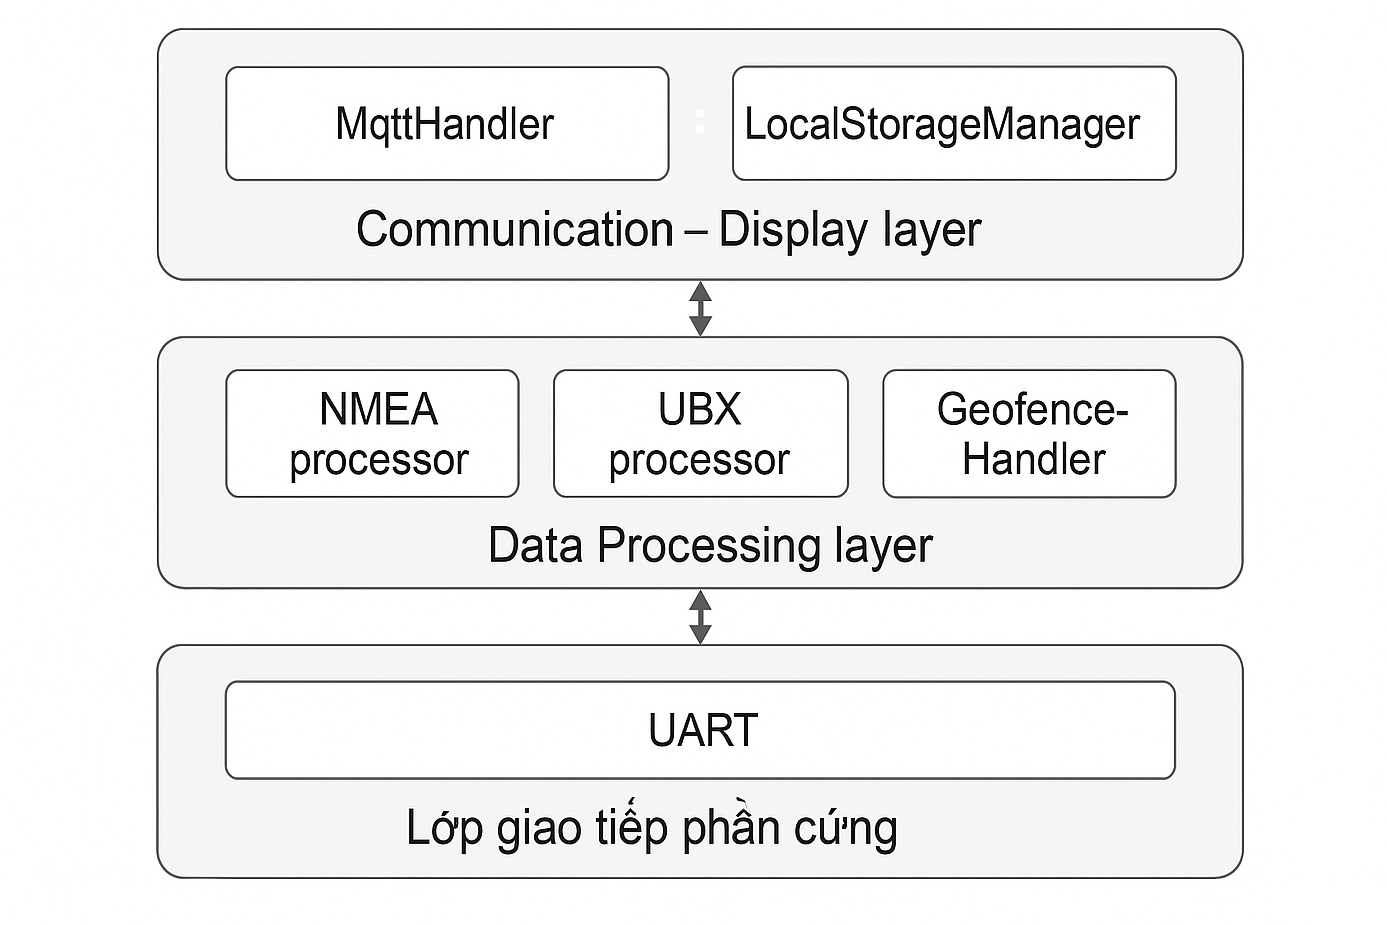
\includegraphics[width=0.8\textwidth]{Hinhve/System.png}
    \caption{Mô hình phân lớp}
\end{figure}


\label{subsection:4.2.1}
\subsection{Lớp giao tiếp phần cứng}
\label{subsection:4.2.2}
Lớp giao tiếp phần cứng là lớp nền trong toàn bộ kiến trúc phần mềm, chịu trách nhiệm kết nối với thiết bị GNSS và thu nhận dữ liệu thông qua giao tiếp UART. Thành phần trung tâm trong lớp này là lớp \text{UartReader}, được xây dựng để thực hiện các thao tác mở cổng, đọc dữ liệu byte theo thời gian thực và gửi dữ liệu điều khiển xuống thiết bị.

Ngay khi thiết bị khởi động, ứng dụng sử dụng \text{UartReader} để mở cổng UART tại đường dẫn cấu hình sẵn (\text{/dev/ttyHSL0}). Nếu mở cổng thành công, một luồng xử lý riêng sẽ được kích hoạt để liên tục đọc từng byte từ thiết bị GNSS. Mỗi byte nhận được sẽ được chuyển vào chuỗi xử lý kế tiếp thông qua các lớp phân tích dữ liệu.

Luồng xử lý dữ liệu sau khi nhận byte từ UART được chia thành hai nhánh chính, tương ứng với hai định dạng bản tin phổ biến của thiết bị GNSS là NMEA và UBX. Nếu dữ liệu là bản tin NMEA, tức có ký tự bắt đầu là dấu \text{\$}, luồng byte sẽ được chuyển đến lớp \text{NMEAProcessor} để tái tạo thành một chuỗi hoàn chỉnh. Sau đó, chuỗi này được phân tích bởi lớp \text{NMEAHandler} nhằm trích xuất thông tin định vị như toạ độ, tốc độ di chuyển, hướng đi và tính hợp lệ của tín hiệu.

Ngược lại, nếu byte đầu là cặp \text{0xB5 0x62} thì dữ liệu thuộc định dạng UBX. Lúc này, nó sẽ được truyền đến các bộ xử lý như \text{GNSSProcessor}, \text{NavStatusProcessor} hoặc \text{SFRBXProcessor} để kiểm tra độ dài, xác thực checksum và phân tích phần nội dung payload. Các bộ xử lý này hỗ trợ việc trích xuất thông tin cấu hình GNSS hoặc trạng thái vệ tinh đang hoạt động.

Dữ liệu định vị hợp lệ sau khi được trích xuất sẽ được chuyển tiếp lên lớp xử lý trung gian để tính trung bình toạ độ, phát hiện ra các vi phạm geofence hoặc gửi thông tin đến nền tảng ThingsBoard thông qua giao thức MQTT. Bên cạnh chức năng đọc, lớp giao tiếp phần cứng còn cho phép gửi dữ liệu điều khiển xuống thiết bị GNSS. Chẳng hạn, lớp \text{GNSSControl} có thể tạo bản tin \text{UBX-CFG-GNSS} để bật hoặc tắt các hệ thống vệ tinh như GPS, GLONASS, Galileo hoặc BeiDou. Bản tin sau đó được gửi đi thông qua UART nhờ phương thức ghi của \text{UartReader}.

Luồng xử lý UART đảm bảo rằng dữ liệu GNSS được tiếp nhận liên tục và chính xác, bất kể trong điều kiện hoạt động bình thường hay gián đoạn mạng. Đây là bước đầu tiên và cũng là tiền đề quan trọng để hệ thống thực hiện các tác vụ giám sát, phân tích và truyền thông một cách ổn định, đáng tin cậy.

\begin{figure}[H]
    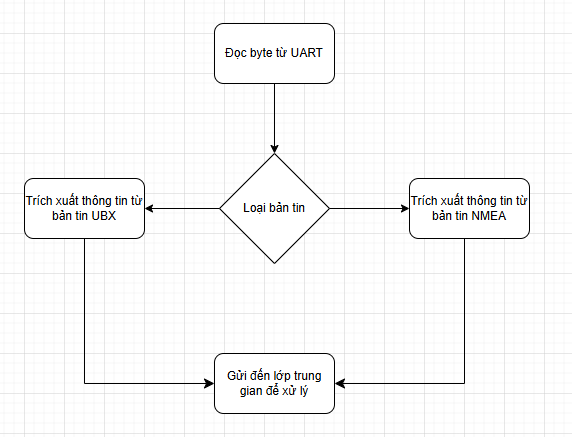
\includegraphics[width=\linewidth]{Hinhve/HardwareFlow.png}
    \caption{Luồng xử lý dữ liệu lớp phần cứng}
    \label{fig:label}
\end{figure}

\subsection{Lớp xử lý dữ liệu}
\label{subsection:4.2.3}
Lớp xử lý dữ liệu đóng vai trò trung gian trong hệ thống, đảm nhận nhiệm vụ tiếp nhận dữ liệu thô từ lớp giao tiếp phần cứng, sau đó phân tích, trích xuất và xử lý thông tin định vị cần thiết. Lớp này được cấu trúc thành nhiều mô-đun chức năng, mỗi mô-đun đảm nhận một nhiệm vụ chuyên biệt tương ứng với các loại bản tin định vị khác nhau.
\subsubsection{Các bản tin từ module GNSS ublox NEO-M9}
\label{subsubsection:4.2.3.1}
Module GNSS u-blox NEO-M9 hỗ trợ truyền dữ liệu định vị qua hai định dạng bản tin chính là NMEA và UBX. Bản tin NMEA được sử dụng phổ biến để cung cấp thông tin vị trí dưới dạng chuỗi ASCII, trong khi bản tin UBX là định dạng nhị phân độc quyền của u-blox, cho phép truyền thông tin cấu hình và trạng thái với độ chính xác và linh hoạt cao hơn. Hệ thống phần mềm sử dụng bốn bản tin chính: \text{NMEA-RMC}, \text{UBX-CFG-GNSS}, \text{UBX-NAV-STATUS} và \text{UBX-RXM-SFRBX}, với chức năng và cấu trúc như sau:

Bản tin \text{RMC} (Recommended Minimum Specific GNSS Data) cung cấp thông tin tối thiểu cần thiết về định vị như thời gian, vị trí, tốc độ và hướng. Chuỗi bắt đầu bằng \text{\$GxRMC} và kết thúc bằng checksum. Các trường trong bản tin có định dạng văn bản, phân tách bằng dấu phẩy.

\begin{longtable}{|c|l|l|l|l|p{4cm}|}
\hline
\textbf{Field} & \textbf{Tên trường} & \textbf{Định dạng} & \textbf{Đơn vị} & \textbf{Ví dụ} & \textbf{Mô tả} \\
\hline
\endfirsthead

\hline
\textbf{Field} & \textbf{Tên trường} & \textbf{Định dạng} & \textbf{Đơn vị} & \textbf{Ví dụ} & \textbf{Mô tả} \\
\hline
\endhead

\hline
\endfoot

\endlastfoot

0 & xxRMC & Chuỗi & - & GPRMC & Mã tin nhắn RMC \\ \hline
1 & Thời gian & hhmmss.sss & - & 083559.00 & Thời gian UTC \\ \hline
2 & Trạng thái & Ký tự & - & A & Trạng thái tín hiệu (A = hợp lệ) \\ \hline
3 & Vĩ độ & ddmm.mmmm & Độ & 4717.11437 & Vĩ độ \\ \hline
4 & NS & Ký tự & - & N & Chỉ báo Bắc - Nam \\ \hline
5 & Kinh độ & dddmm.mmmm & Độ & 00833.91522 & Kinh độ \\ \hline
6 & EW & Ký tự & - & E & Chỉ báo Đông - Tây \\ \hline
7 & Tốc độ & float & knots & 22.4 & Tốc độ mặt đất \\ \hline
8 & Hướng đi & float & Độ & 84.4 & Hướng chuyển động \\ \hline
9 & Ngày & ddmmyy & - & 230394 & Ngày tháng năm \\ \hline
10 & mv & Số & Độ & - & Biến thiên từ trường \\ \hline
11 & mvEW & Ký tự & - & - & Biến thiên từ trường Đông - Tây \\ \hline
12 & posMode & Ký tự & - & A & Chỉ báo chế độ \\ \hline
13 & navStatus & Ký tự & - & V & Trạng thái định vị \\ \hline
14 & cs & Thập lục phân & - & 57 & Checksum \\ \hline
15 & CRLF & Ký tự & - & - & Ký tự xuống dòng \\ \hline

\caption{Cấu trúc bản tin NMEA-RMC} \\
\end{longtable}

Bản tin VTG (Course Over Ground and Ground Speed) cung cấp thông tin về hướng di chuyển và tốc độ của thiết bị so với mặt đất. Chuỗi bản tin này bắt đầu bằng ký hiệu \text{\$GxVTG} và kết thúc bằng mã kiểm tra lỗi (checksum). Các trường dữ liệu trong bản tin có định dạng văn bản, được phân tách bằng dấu phẩy.


\begin{longtable}{|c|l|l|l|l|p{4cm}|}
\hline
\textbf{Field} & \textbf{Tên trường} & \textbf{Định dạng} & \textbf{Đơn vị} & \textbf{Ví dụ} & \textbf{Mô tả} \\
\hline
\endfirsthead

\hline
\textbf{Field} & \textbf{Tên trường} & \textbf{Định dạng} & \textbf{Đơn vị} & \textbf{Ví dụ} & \textbf{Mô tả} \\
\hline
\endhead

\hline
\endfoot

\endlastfoot

0 & xxVTG & Chuỗi & - & GPVTG & Mã bản tin VTG (xx là Talker ID) \\ \hline
1 & cogt & Số thực & Độ & 77.52 & Hướng di chuyển mặt đất (đúng theo phương vị thực) \\ \hline
2 & cogtUnit & Ký tự & - & T & Đơn vị hướng: T = True (cố định) \\ \hline
3 & cogm & Số thực & Độ & - & Hướng di chuyển mặt đất (theo phương vị từ, nếu có) \\ \hline
4 & cogmUnit & Ký tự & - & M & Đơn vị hướng: M = Magnetic (cố định) \\ \hline
5 & sogn & Số thực & knots & 0.004 & Tốc độ di chuyển mặt đất theo đơn vị knots \\ \hline
6 & sognUnit & Ký tự & - & N & Đơn vị tốc độ: N = knots (cố định) \\ \hline
7 & sogk & Số thực & km/h & 0.008 & Tốc độ di chuyển mặt đất theo đơn vị km/h \\ \hline
8 & sogkUnit & Ký tự & - & K & Đơn vị tốc độ: K = kilometer/hour (cố định) \\ \hline
9 & posMode & Ký tự & - & A & Chỉ báo chế độ định vị (xuất hiện từ phiên bản NMEA 2.3 trở lên) \\ \hline
10 & cs & Thập lục phân & - & 06 & Checksum để kiểm tra lỗi \\ \hline
11 & CRLF & Ký tự & - & - & Ký tự xuống dòng kết thúc bản tin \\ \hline

\caption{Cấu trúc bản tin NMEA-VTG} \\
\end{longtable}

Bản tin \text{GNS} (GNSS Fix Data) cung cấp thông tin về toạ độ định vị, trạng thái tín hiệu và số lượng vệ tinh được sử dụng từ các hệ thống GNSS. Chuỗi bắt đầu bằng \text{\$GxGNS} và kết thúc bằng checksum. Các trường trong bản tin có định dạng văn bản, phân tách bằng dấu phẩy.

\begin{longtable}{|c|l|l|l|l|p{4cm}|}
\hline
\textbf{Field} & \textbf{Tên trường} & \textbf{Định dạng} & \textbf{Đơn vị} & \textbf{Ví dụ} & \textbf{Mô tả} \\
\hline
\endfirsthead

\hline
\textbf{Field} & \textbf{Tên trường} & \textbf{Định dạng} & \textbf{Đơn vị} & \textbf{Ví dụ} & \textbf{Mô tả} \\
\hline
\endhead

\hline
\endfoot

\endlastfoot

0 & xxGGA & Chuỗi & - & GPGGA & Mã bản tin GGA (xx là Talker ID) \\ \hline
1 & time & hhmmss.ss & - & 092725.00 & Thời gian UTC \\ \hline
2 & lat & ddmm.mmmmm & Độ & 4717.11399 & Vĩ độ (độ và phút) \\ \hline
3 & NS & Ký tự & - & N & Chỉ báo Bắc/Nam \\ \hline
4 & lon & dddmm.mmmmm & Độ & 00833.91590 & Kinh độ (độ và phút) \\ \hline
5 & EW & Ký tự & - & E & Chỉ báo Đông/Tây \\ \hline
6 & quality & Chữ số & - & 1 & Chất lượng tín hiệu định vị \\ \hline
7 & numSV & Số & - & 08 & Số vệ tinh sử dụng (0–12) \\ \hline
8 & HDOP & Số thực & - & 1.01 & Độ phân giải theo phương ngang \\ \hline
9 & alt & Số thực & m & 499.6 & Độ cao so với mực nước biển trung bình \\ \hline
10 & altUnit & Ký tự & - & M & Đơn vị độ cao: mét (cố định) \\ \hline
11 & sep & Số thực & m & 48.0 & Độ lệch địa hình giữa ellipsoid và mực nước biển \\ \hline
12 & sepUnit & Ký tự & - & M & Đơn vị độ lệch địa hình: mét (cố định) \\ \hline
13 & diffAge & Số & s & - & Độ tuổi hiệu chỉnh sai số (nếu có) \\ \hline
14 & diffStation & Số & - & - & Mã trạm phát hiệu chỉnh (nếu có) \\ \hline
15 & cs & Thập lục phân & - & 5B & Checksum để kiểm tra lỗi \\ \hline
16 & CRLF & Ký tự & - & - & Ký tự xuống dòng kết thúc bản tin \\ \hline

\caption{Cấu trúc bản tin NMEA-GGA} \\
\end{longtable}


Bản tin \text{GNS} (GNSS Fix Data) cung cấp thông tin về vị trí, trạng thái tín hiệu và số lượng vệ tinh được sử dụng từ các hệ thống định vị toàn cầu. Chuỗi bắt đầu bằng \text{\$GxGNS} và kết thúc bằng checksum. Các trường trong bản tin có định dạng văn bản, phân tách bằng dấu phẩy.

\begin{longtable}{|c|l|l|l|l|p{4cm}|}
\hline
\textbf{Field} & \textbf{Tên trường} & \textbf{Định dạng} & \textbf{Đơn vị} & \textbf{Ví dụ} & \textbf{Mô tả} \\
\hline
\endfirsthead

\hline
\textbf{Field} & \textbf{Tên trường} & \textbf{Định dạng} & \textbf{Đơn vị} & \textbf{Ví dụ} & \textbf{Mô tả} \\
\hline
\endhead

\hline
\endfoot

\endlastfoot

0 & xxGNS & Chuỗi & - & GPGNS & Mã bản tin GNS (xx là Talker ID) \\ \hline
1 & time & hhmmss.ss & - & 091547.00 & Thời gian UTC \\ \hline
2 & lat & ddmm.mmmmm & Độ & 5114.50897 & Vĩ độ (độ và phút) \\ \hline
3 & NS & Ký tự & - & N & Chỉ báo Bắc/Nam \\ \hline
4 & lon & dddmm.mmmmm & Độ & 00012.28663 & Kinh độ (độ và phút) \\ \hline
5 & EW & Ký tự & - & E & Chỉ báo Đông/Tây \\ \hline
6 & posMode & Ký tự & - & AAAA & Chế độ định vị của từng hệ GNSS (GPS, GLONASS, Galileo, BeiDou) \\ \hline
7 & numSV & Số & - & 10 & Số lượng vệ tinh được sử dụng (0–99) \\ \hline
8 & HDOP & Số thực & - & 0.83 & Độ phân giải theo phương ngang \\ \hline
9 & alt & Số thực & m & 111.1 & Độ cao so với mực nước biển trung bình \\ \hline
10 & sep & Số thực & m & 45.6 & Độ lệch địa hình giữa ellipsoid và mực nước biển \\ \hline
11 & diffAge & Số & s & - & Độ tuổi hiệu chỉnh sai số (nếu có) \\ \hline
12 & diffStation & Số & - & - & Mã trạm phát hiệu chỉnh (nếu có) \\ \hline
13 & navStatus & Ký tự & - & V & Trạng thái điều hướng (có trong NMEA 4.10 trở lên) \\ \hline
14 & cs & Thập lục phân & - & 71 & Checksum để kiểm tra lỗi \\ \hline
15 & CRLF & Ký tự & - & - & Ký tự xuống dòng kết thúc bản tin \\ \hline

\caption{Cấu trúc bản tin NMEA-GNS} \\
\end{longtable}

Bản tin \text{UBX-CFG-GNSS} được sử dụng để cấu hình hệ thống GNSS đang hoạt động trên thiết bị. Bản tin chứa thông tin về số lượng kênh theo phần cứng và phần mềm, số hệ thống GNSS được cấu hình và trạng thái bật/tắt của từng hệ thống.

\begin{table}[H]
\centering
\begin{tabular}{|c|l|l|l|l|p{6cm}|}
\hline
\textbf{Offset} & \textbf{Tên trường} & \textbf{Định dạng} & \textbf{Đơn vị} & \textbf{Ví dụ} & \textbf{Mô tả} \\
\hline
0 & msgVer & uint8 & - & 0 & Phiên bản bản tin \\
\hline
1 & numTrkChHw & uint8 & kênh & 32 & Số kênh phần cứng hỗ trợ \\
\hline
2 & numTrkChUse & uint8 & kênh & 32 & Số kênh GNSS được sử dụng \\
\hline
3 & numConfigBlocks & uint8 & - & 6 & Số hệ thống GNSS được cấu hình \\
\hline
4 & repeated blocks & struct & - & ... & Dữ liệu cấu hình cho từng hệ thống GNSS (ID, số kênh, cờ enable, flags, v.v.) \\
\hline
\end{tabular}
\caption{Cấu trúc bản tin UBX-CFG-GNSS}
\end{table}

Bản tin \texttt{UBX-NAV-STATUS} cung cấp thông tin về trạng thái định vị hiện tại của thiết bị, bao gồm kiểu fix, các cờ trạng thái, và thông tin xác thực tín hiệu.

\begin{table}[H]
\centering
\begin{tabular}{|c|l|l|l|l|p{6cm}|}
\hline
\textbf{Offset} & \textbf{Tên trường} & \textbf{Định dạng} & \textbf{Đơn vị} & \textbf{Ví dụ} & \textbf{Mô tả} \\
\hline
0 & iTOW & uint32 & ms & 501867000 & Thời gian GPS (Time of Week) \\
\hline
4 & gpsFix & uint8 & - & 3 & Trạng thái định vị (3 = 3D fix) \\
\hline
5 & flags & bitfield & - & 0x0D & Các cờ phản ánh chất lượng và độ tin cậy tín hiệu \\
\hline
6 & fixStat & bitfield & - & 0x00 & Trạng thái xác định vị trí \\
\hline
7 & flags2 & bitfield & - & 0x00 & Các cờ bổ sung \\
\hline
\end{tabular}
\caption{Cấu trúc bản tin UBX-NAV-STATUS}
\end{table}

Bản tin \texttt{UBX-RXM-SFRBX} chứa dữ liệu thô từ tín hiệu vệ tinh, thường được sử dụng cho mục đích phân tích tín hiệu ở lớp thấp. Bản tin cung cấp thông tin như ID vệ tinh, tần số và các từ dữ liệu 32 bit từ mỗi vệ tinh.

\begin{table}[H]
\centering
\begin{tabular}{|c|l|l|l|l|p{6cm}|}
\hline
\textbf{Offset} & \textbf{Tên trường} & \textbf{Định dạng} & \textbf{Đơn vị} & \textbf{Ví dụ} & \textbf{Mô tả} \\
\hline
0 & gnssId & uint8 & - & 0 & ID hệ thống GNSS (0 = GPS) \\
\hline
1 & svId & uint8 & - & 3 & ID vệ tinh \\
\hline
2 & reserved1 & uint8 & - & 0 & Trường dự phòng \\
\hline
3 & freqId & uint8 & - & 0 & ID tần số tín hiệu \\
\hline
4 & numWords & uint8 & - & 10 & Số lượng từ dữ liệu GNSS \\
\hline
8 & dwrd & uint32[10] & - & ... & Dữ liệu 32 bit từ tín hiệu vệ tinh \\
\hline
\end{tabular}
\caption{Cấu trúc bản tin UBX-RXM-SFRBX}
\end{table}


\subsubsection{Luồng xử lý dữ liệu}
\label{subsubsection:4.2.3.2}
Lớp xử lý dữ liệu đóng vai trò trung gian trong hệ thống, đảm nhận nhiệm vụ tiếp nhận dữ liệu thô từ lớp giao tiếp phần cứng, sau đó phân tích, trích xuất và xử lý thông tin định vị cần thiết. Lớp này được cấu trúc thành nhiều mô-đun chức năng, mỗi mô-đun đảm nhận một nhiệm vụ chuyên biệt tương ứng với các loại bản tin định vị khác nhau.

Đối với dữ liệu NMEA, sau khi được tái dựng thành chuỗi hoàn chỉnh, chuỗi này sẽ được truyền vào lớp \text{NMEAHandler} để trích xuất các thông tin như vĩ độ, kinh độ, tốc độ di chuyển và trạng thái tín hiệu. Việc xử lý các câu lệnh \text{GGA}, \text{GNS}, \tett{RMC}, hoặc \text{VTG} được thực hiện thông qua các parser chuyên biệt, giúp đảm bảo khả năng trích xuất chính xác từ đa nguồn GNSS.

Trong trường hợp bản tin có định dạng UBX, hệ thống sử dụng các mô-đun chuyên biệt như \text{GNSSProcessor}, \text{NavStatusProcessor} và \text{SFRBXProcessor}. Các mô-đun này thực hiện việc nhận diện chuỗi bản tin, kiểm tra độ dài hợp lệ, xác thực checksum và trích xuất thông tin cấu hình hoặc trạng thái vệ tinh. Thông tin này phục vụ cho việc xác định số lượng hệ thống GNSS đang hoạt động, theo dõi chất lượng tín hiệu hoặc tái cấu hình hoạt động GNSS thông qua các bản tin điều khiển.

Sau khi dữ liệu được phân tích và xác thực, lớp xử lý tiếp tục thực hiện các thao tác cao hơn như tính tốc độ di chuyển dựa trên thời gian thực và khoảng cách giữa các toạ độ, xác định thay đổi vị trí vượt quá ngưỡng cấu hình, hoặc phát hiện sự thay đổi trạng thái hoạt động của GNSS. Các dữ liệu hợp lệ được truyền đến lớp truyền thông để hiển thị hoặc đồng bộ với nền tảng giám sát.

Một chức năng quan trọng khác của lớp xử lý dữ liệu là cơ chế geofence, cho phép hệ thống phát hiện khi thiết bị di chuyển ra ngoài phạm vi khu vực đã được định nghĩa từ trước. Các khu vực này được biểu diễn dưới dạng tập hợp các đỉnh tạo thành một đa giác khép kín, thường tương ứng với ranh giới hành chính như tỉnh hoặc thành phố. Tọa độ hiện tại của thiết bị, sau khi được trích xuất và xác thực, sẽ được chuyển đến mô-đun GeofenceHandler để kiểm tra xem điểm đó có nằm trong vùng giới hạn hay không.

Thuật toán được sử dụng là thuật toán tia cắt (ray casting algorithm), hoạt động theo nguyên lý đếm số lần một tia xuất phát từ điểm cần kiểm tra cắt các cạnh của đa giác. Nếu số lần cắt là số lẻ, điểm được xác định là nằm trong vùng; ngược lại, nếu là số chẵn, điểm nằm ngoài. Trong quá trình xử lý, thuật toán cũng bao gồm cơ chế hiệu chỉnh để tránh các trường hợp biên gây ra sai số, ví dụ như khi điểm trùng với một đỉnh của đa giác hoặc nằm trên một cạnh ngang. Điều này giúp tăng độ tin cậy của quá trình xác định vị trí tương đối của thiết bị với khu vực cấu hình.

Kết quả kiểm tra geofence sẽ được sử dụng để tạo các bản tin cảnh báo, thông qua đó nền tảng ThingsBoard có thể hiển thị trạng thái thiết bị như "bên trong" hoặc "bên ngoài" vùng theo thời gian thực. Nếu thiết bị nằm ngoài vùng giới hạn, hệ thống sẽ gửi một thuộc tính isOutside = true lên server. Khi thiết bị quay lại vùng an toàn, giá trị này sẽ được cập nhật lại. Nhờ cơ chế này, hệ thống có thể hỗ trợ các ứng dụng yêu cầu giám sát chặt chẽ vị trí như theo dõi phương tiện, quản lý nhân lực hoặc cảnh báo vi phạm khu vực an toàn.

Ngoài ra, để đảm bảo hoạt động ổn định trong môi trường mạng không liên tục, các bản ghi dữ liệu định vị sẽ được lưu tạm thời bằng lớp \text{LocalStorageManager}. Khi mạng ổn định trở lại, dữ liệu này sẽ được đồng bộ qua lớp truyền thông MQTT. Cơ chế này giúp tránh mất dữ liệu trong quá trình thiết bị di chuyển qua các khu vực có chất lượng kết nối kém.

Toàn bộ lớp xử lý dữ liệu được thiết kế theo hướng mở rộng và tương thích với nhiều loại bản tin GNSS khác nhau, đảm bảo hiệu quả phân tích và tính linh hoạt trong các tình huống vận hành thực tế.
\subsection{Lớp truyền thông}
\label{subsection:4.2.4}
Lớp truyền thông có vai trò kết nối giữa thiết bị và nền tảng ThingsBoard thông qua giao thức MQTT. Thành phần trung tâm của lớp này là lớp \text{MqttHandler}, chịu trách nhiệm khởi tạo kết nối, gửi dữ liệu định vị, gửi các thông số trạng thái hệ thống và tiếp nhận các cấu hình điều khiển từ xa. 

Ngay khi khởi động, \text{MqttHandler} tiến hành kết nối đến máy chủ MQTT bằng định danh thiết bị ThingsBoard. Sau khi kết nối thành công, thiết bị sẽ tự động gửi một bản tin \text{init} chứa các thuộc tính cấu hình hiện tại của thiết bị.

Chương trình sử dụng hai topic chính: \text{telemetryTopic} để gửi dữ liệu thời gian thực như toạ độ và tốc độ di chuyển và \text{attributeTopic} để gửi hoặc nhận các thuộc tính cấu hình hệ thống như trạng thái pin, geofence hoặc điều kiện hoạt động. Tùy theo chế độ định vị, hệ thống sử dụng hai chế độ gửi dữ liệu:
\begin{itemize}
    \item \text{DEVICE\_LOCATION}: gửi tọa độ từ dịch vụ định vị của Android.
    \item \text{UBLOX\_LOCATION}: gửi tọa độ GNSS trung bình từ module u-blox.
\end{itemize}

Để tối ưu hiệu suất truyền thông và tiết kiệm năng lượng, lớp này chỉ gửi dữ liệu khi thiết bị có kết nối mạng hoặc khi tọa độ thay đổi vượt qua ngưỡng cấu hình. Nếu mất mạng, dữ liệu sẽ được lưu tạm thời trong bộ nhớ cục bộ thông qua lớp \text{LocalStorageManager} và tự động đồng bộ lại khi mạng ổn định trở lại.

Ngoài dữ liệu định vị, \text{MqttHandler} cũng xử lý các bản tin phản hồi từ ThingsBoard. Các bản tin thuộc chủ đề thuộc tính (\texttt{attribute}) được phân tích và cập nhật trực tiếp vào các thông số hoạt động như khoảng cách tối đa (\text{maxDistance}), thời gian tối đa (\text{maxTimeout}), tên tỉnh giám sát hoặc trạng thái bật/tắt vùng geofence. Nếu geofence được bật, ranh giới địa lý tương ứng với tỉnh được lấy từ file \text{provinces.json} và gửi ngược lên server để hiển thị trên dashboard.

Cuối cùng, lớp này còn hỗ trợ gửi các thuộc tính trạng thái như mức pin, trạng thái sạc, trạng thái GPS và cờ xác định thiết bị có nằm ngoài khu vực địa lý không (\text{isOutside}). Toàn bộ lớp được thiết kế bất đồng bộ, với cơ chế tự động kết nối lại khi xảy ra gián đoạn để đảm bảo tính liên tục trong quá trình truyền nhận dữ liệu.


\section{Phần mềm nhúng trên vi điều khiển ATmega8}
\label{section:4.3}
Phần mềm nhúng trên vi điều khiển ATmega8 đóng vai trò trung gian điều phối giữa các cảm biến vật lý và thiết bị Android, nhằm đảm bảo hệ thống chỉ được kích hoạt khi thực sự cần thiết. Cụ thể, ATmega8 giám sát tín hiệu từ cảm biến rung để phát hiện sự hiện diện hoặc hoạt động của người dùng. Khi có tín hiệu chuyển động, vi điều khiển thực hiện thao tác cấp nguồn và khởi động thiết bị Android. Ngược lại, nếu không còn chuyển động trong một khoảng thời gian định trước, hệ thống sẽ chủ động ngắt nguồn và đưa thiết bị về trạng thái tiết kiệm năng lượng.

Chương này trình bày chi tiết thiết kế và triển khai phần mềm nhúng cho ATmega8, bao gồm cấu hình các chân I/O, thiết lập ngắt ngoài, lựa chọn và cài đặt chế độ tiết kiệm năng lượng phù hợp, cùng với mô hình điều khiển theo máy trạng thái. Thiết kế này cho thấy sự cân bằng giữa hiệu quả sử dụng năng lượng và khả năng đáp ứng nhanh với các sự kiện ngoài môi trường, góp phần nâng cao độ bền và tính ổn định cho toàn bộ hệ thống.
\subsection{Cấu hình các chân GPIO trên vi điều khiển ATmega8}
\label{subsection:4.3.1}
GPIO (General Purpose Input/Output) là các chân vào/ra mục đích chung cho phép vi điều khiển trao đổi tín hiệu số với các thiết bị ngoại vi. Các chân này có thể được thiết lập để hoạt động ở chế độ đầu vào (nhận tín hiệu) hoặc đầu ra (phát tín hiệu). Trong các hệ thống nhúng, GPIO đóng vai trò quan trọng trong việc điều khiển thiết bị, nhận tín hiệu điều kiện hoặc phản hồi trạng thái. Trên vi điều khiển ATmega8, toàn bộ các chân của các cổng I/O như PORTB, PORTC và PORTD đều có thể được sử dụng như các GPIO đa năng. Điều này giúp lập trình viên có khả năng cấu hình linh hoạt tùy theo yêu cầu phần cứng và chức năng ứng dụng.


Để cấu hình và vận hành các chân GPIO, ATmega8 cung cấp ba thanh ghi điều khiển chính cho mỗi cổng:

\begin{itemize}
    \item \textbf{DDRx (Data Direction Register)}: đây là thanh ghi 8 bit dùng để xác định hướng dữ liệu của từng chân trong cổng. Nếu bit tại vị trí tương ứng được ghi là 1, chân đó sẽ được cấu hình là đầu ra. Ngược lại, nếu bit đó bằng 0, chân sẽ được cấu hình là đầu vào. Ví dụ, thiết lập \text{DDRC |= (1 << PC0);} sẽ cấu hình chân PC0 là đầu ra.
    
    \item \textbf{PORTx}: thanh ghi này có vai trò khác nhau tùy thuộc vào hướng của chân. 
    \begin{itemize}
        \item Nếu chân đang được cấu hình là đầu ra, ghi giá trị logic 1 vào bit tương ứng sẽ đặt chân ở mức cao (logic HIGH), còn ghi giá trị 0 sẽ đặt ở mức thấp (logic LOW). Ví dụ, \text{PORTC |= (1 << PC0);} sẽ kéo chân PC0 lên mức cao.
        \item Nếu chân đang ở chế độ đầu vào, ghi giá trị 1 vào bit tương ứng sẽ bật điện trở kéo lên nội (pull-up), giúp đảm bảo tín hiệu ổn định khi không có tác động ngoại vi. Ví dụ, \text{PORTD |= (1 << PD3);} sẽ bật pull-up cho chân PD3 khi đang là đầu vào.
    \end{itemize}

    \item \textbf{PINx}: đây là thanh ghi chỉ đọc, cho phép kiểm tra mức logic hiện tại tại các chân. Thường được dùng trong xử lý tín hiệu từ cảm biến hoặc nút nhấn. Ví dụ, \text{if (PIND \& (1 << PD3))} sẽ trả về đúng nếu chân PD3 đang ở mức cao.
\end{itemize}

Trong đồ án này, các chân GPIO của ATmega8 được sử dụng để điều khiển các chức năng quan trọng của hệ thống giám sát. Cụ thể, có bốn chân được sử dụng và được cấu hình như sau:

\begin{itemize}
    \item \textbf{Chân PC0 (PWRKEY):} được cấu hình là \textbf{đầu ra (output)}. Chân này được kết nối với chân điều khiển PWRKEY của thiết bị Android để thực hiện thao tác bật hoặc tắt thiết bị. Trạng thái ban đầu của chân này được đặt ở mức logic thấp (\text{PORTC \&= \string~(1 << PC0)}), đảm bảo thiết bị không bị kích hoạt khi hệ thống mới khởi động.
    
    \item \textbf{Chân PC1 (LED):} được cấu hình là \textbf{đầu ra (output)}. Đây là chân điều khiển đèn LED dùng để hiển thị trạng thái hoạt động của hệ thống. Khi chân này ở mức cao, đèn LED sẽ sáng, biểu thị rằng hệ thống đang ở trạng thái bật. Trạng thái ban đầu được thiết lập ở mức logic thấp để LED tắt khi chưa có sự kiện kích hoạt.

    \item \textbf{Chân PB1 (UBLOX):} được cấu hình là \textbf{đầu ra (output)}. Chân này điều khiển đường cấp nguồn cho module định vị GNSS u-blox. Khi chân này được đặt ở mức cao, nguồn cho module GNSS sẽ được cấp. Trạng thái khởi tạo được đặt ở mức thấp, tức là module GNSS chưa được cấp nguồn khi hệ thống khởi động.
    
    \item \textbf{Chân PD3 (INPUT):} được cấu hình là \textbf{đầu vào (input)}. Đây là chân kết nối với cảm biến chuyển động (ví dụ cảm biến rung) nhằm phát hiện có hoạt động từ môi trường bên ngoài. Khi cảm biến phát hiện chuyển động, chân này sẽ chuyển sang mức cao. Để đảm bảo tín hiệu ổn định khi không có tác động, điện trở kéo lên nội được bật thông qua việc ghi giá trị 1 vào bit tương ứng trong thanh ghi \text{PORTD}.
\end{itemize}

Cách cấu hình này đảm bảo rằng mỗi chân đều có chức năng rõ ràng, định hướng hoạt động cụ thể và được khởi tạo với trạng thái an toàn. Điều này giúp hệ thống vận hành ổn định và phản hồi chính xác theo các tín hiệu đầu vào cũng như yêu cầu điều khiển đầu ra. Các thiết bị được kết nối sẽ chỉ hoạt động khi có điều kiện thích hợp, tránh tiêu tốn năng lượng không cần thiết hoặc phát sinh lỗi trong quá trình khởi động.

Việc cấu hình các chân này được thực hiện trong hàm \text{setup\_io()} với các bước như sau:

\begin{itemize}
    \item Các chân \textbf{PC0}, \textbf{PC1} và \textbf{PB1} được thiết lập làm đầu ra bằng cách ghi giá trị 1 vào các bit tương ứng trong các thanh ghi \text{DDRC} và \text{DDRB}.
    \item Trạng thái ban đầu của các chân đầu ra được đặt ở mức logic thấp bằng cách ghi giá trị 0 vào các bit tương ứng trong \text{PORTC} và \text{PORTB}, giúp tránh kích hoạt ngoài ý muốn sau khi khởi động hệ thống.
    \item Chân \textbf{PD3} được cấu hình làm đầu vào bằng cách ghi giá trị 0 vào bit tương ứng trong \text{DDRD}, đồng thời bật điện trở kéo lên nội bằng cách ghi 1 vào bit tương ứng trong \text{PORTD}.
\end{itemize}

Việc bật điện trở kéo lên nội cho chân đầu vào là cần thiết để đảm bảo tín hiệu ổn định trong trạng thái nghỉ, tránh hiện tượng trôi logic. Cách cấu hình nêu trên đảm bảo rằng hệ thống có trạng thái xác định, đáng tin cậy và sẵn sàng hoạt động chính xác ngay từ thời điểm khởi động. Điều này góp phần quan trọng vào độ ổn định và tính đúng đắn trong điều khiển thiết bị Android theo điều kiện thực tế.

\subsection{Cơ chế ngắt và cấu hình ngắt trên ATmega8}
\label{section:4.3.2}

Cơ chế ngắt (interrupt) là một phần tử quan trọng trong thiết kế hệ thống nhúng, giúp vi điều khiển có khả năng phản ứng tức thời với các sự kiện bất đồng bộ từ môi trường. Ngắt cho phép hệ thống tạm dừng chương trình đang thực thi để xử lý một sự kiện khẩn cấp, sau đó tiếp tục lại đúng vị trí bị tạm dừng. Điều này làm giảm độ trễ phản hồi và tiết kiệm tài nguyên so với việc kiểm tra liên tục (polling) trạng thái các thiết bị.

Quá trình xử lý ngắt diễn ra theo các bước cơ bản sau:

\begin{itemize}
    \item \textbf{Bước 1:} Một điều kiện ngắt được phát sinh, ví dụ: tín hiệu từ cảm biến, bộ định thời tràn, dữ liệu được nhận qua UART, v.v.
    \item \textbf{Bước 2:} Vi điều khiển kiểm tra xem ngắt đó có được cho phép không (bit enable của ngắt có được bật và ngắt toàn cục đã được cho phép bằng lệnh \text{sei()}).
    \item \textbf{Bước 3:} Nếu ngắt được chấp nhận, vi điều khiển tạm dừng chương trình chính (main), lưu vị trí hiện tại (Program Counter) và nhảy tới hàm xử lý ngắt tương ứng (ISR - Interrupt Service Routine).
    \item \textbf{Bước 4:} ISR được thực hiện. Sau khi hoàn tất, lệnh \text{RETI} (Return from Interrupt) được gọi để khôi phục trạng thái và tiếp tục chương trình chính từ vị trí bị gián đoạn.
\end{itemize}

Cơ chế này đảm bảo rằng hệ thống luôn sẵn sàng phản hồi nhanh chóng mà không cần tiêu tốn thời gian kiểm tra liên tục, đặc biệt hữu ích trong các ứng dụng tiết kiệm năng lượng hoặc thời gian thực.

ATmega8 hỗ trợ nhiều loại ngắt khác nhau, bao phủ toàn bộ các chức năng quan trọng của hệ thống:

\begin{itemize}
    \item \textbf{Ngắt ngoài (External Interrupts):} gồm INT0 (PD2) và INT1 (PD3), có thể cấu hình để kích hoạt theo cạnh lên, cạnh xuống hoặc mức thấp. Dùng để phản ứng với các tín hiệu từ bên ngoài, ví dụ như cảm biến, công tắc, v.v.
    
    \item \textbf{Ngắt thay đổi mức logic (Pin Change Interrupts):} kích hoạt khi bất kỳ chân nào trong một nhóm cụ thể thay đổi trạng thái. Nhóm này không áp dụng được cho tất cả các chân, nhưng giúp mở rộng khả năng giám sát sự thay đổi tín hiệu đầu vào.

    \item \textbf{Ngắt bộ định thời (Timer/Counter Interrupts):}
    \begin{itemize}
        \item Timer0 Overflow (tràn bộ đếm 8-bit)
        \item Timer1 Overflow và Compare Match (cho bộ đếm 16-bit)
        \item Timer2 Overflow
    \end{itemize}
    Dùng để tạo các sự kiện định kỳ, đo thời gian, hoặc điều chế PWM.

    \item \textbf{Ngắt giao tiếp nối tiếp (USART Interrupts):} phát sinh khi có dữ liệu đến hoặc đi qua UART, ví dụ: ngắt nhận ký tự (RXC), ngắt truyền xong (TXC).

    \item \textbf{Ngắt chuyển đổi ADC (ADC Conversion Complete Interrupt):} được kích hoạt khi quá trình chuyển đổi tương tự – số (analog-to-digital) kết thúc.

    \item \textbf{Ngắt Watchdog Timer:} xảy ra khi bộ đếm watchdog hết thời gian mà không được đặt lại, giúp khởi động lại hệ thống nếu chương trình bị treo.
\end{itemize}

Trong phạm vi đồ án này, tôi chỉ sử dụng ngắt ngoài để kiểm soát chế độ của vi điều khiển. Để sử dụng các ngắt ngoài, cần cấu hình các thanh ghi sau:

\begin{itemize}
    \item \textbf{GICR (General Interrupt Control Register):} thanh ghi này cho phép bật ngắt INT0 hoặc INT1. Cụ thể:
    \begin{itemize}
        \item GICR |= (1 << INT1): bật ngắt ngoài INT1.
    \end{itemize}

    \item \textbf{MCUCR (MCU Control Register):} xác định điều kiện kích hoạt ngắt cho INT0 và INT1 bằng hai bit ISCxx:
    \begin{itemize}
        \item ISC11 = 1 và ISC10 = 0: ngắt xảy ra khi có cạnh xuống tại chân INT1 (PD3).
        \item ISC11 = 1 và ISC10 = 1: ngắt xảy ra khi có cạnh lên.
        \item ISC11 = 0 và ISC10 = 0: ngắt xảy ra khi mức thấp liên tục.
    \end{itemize}

    \item \textbf{SREG (Status Register):} chứa bit I - bit cho phép ngắt toàn cục. Để cho phép hệ thống phản hồi ngắt, cần bật bit này bằng lệnh \text{sei()}.
\end{itemize}

Trong đồ án, ngắt INT1 được cấu hình để kích hoạt khi có cạnh xuống tại chân PD3. Điều này phù hợp với nguyên lý hoạt động của cảm biến rung, khi tín hiệu đầu ra chuyển từ mức cao sang thấp để báo hiệu có chuyển động. Việc cấu hình được thực hiện trong hàm \text{setup\_interrupts()} như sau:

\begin{itemize}
    \item Ghi \text{1} vào \text{ISC11} và \text{0} vào \text{ISC10} để chọn chế độ kích hoạt ngắt theo cạnh xuống: \text{MCUCR |= (1 << ISC11);} và \text{MCUCR \&= \string~(1 << ISC10);}
    \item Cho phép ngắt INT1 bằng cách ghi \text{1} vào bit \text{INT1} của thanh ghi \text{GICR}: \text{GICR |= (1 << INT1);}
    \item Kích hoạt ngắt toàn cục bằng lệnh \text{sei();}
\end{itemize}

Trình xử lý ngắt (ISR) cho INT1 được định nghĩa bằng khối \text{ISR(INT1\_vect)}. Trong phiên bản hiện tại, hàm này không thực hiện xử lý cụ thể mà chỉ đóng vai trò duy trì trạng thái sẵn sàng cho việc mở rộng sau này. Tuy nhiên, việc khai báo hàm là cần thiết để tránh lỗi biên dịch và cho phép hệ thống phục hồi đúng trình tự sau khi ngắt kết thúc.

Việc sử dụng ngắt thay vì polling giúp hệ thống tiết kiệm năng lượng khi ở chế độ ngủ và chỉ phản hồi khi có sự kiện thực sự xảy ra, phù hợp với mục tiêu vận hành hiệu quả và ổn định trong môi trường có yêu cầu tiêu thụ điện năng thấp.

\subsection{Cơ chế tiết kiệm năng lượng trên ATmega8}
\label{section:4.3.3}

Trong các hệ thống nhúng hoạt động liên tục hoặc sử dụng nguồn năng lượng hạn chế như pin, việc tối ưu hóa tiêu thụ điện năng đóng vai trò rất quan trọng. Vi điều khiển ATmega8 hỗ trợ nhiều chế độ tiết kiệm năng lượng (power-saving modes) cho phép tạm thời dừng hoặc giới hạn hoạt động của các thành phần bên trong nhằm giảm tiêu thụ dòng. Các chế độ này đặc biệt hiệu quả khi hệ thống không cần xử lý liên tục mà chỉ phản ứng khi có sự kiện từ ngoại vi.

ATmega8 hỗ trợ 4 chế độ tiết kiệm năng lượng chính, được thiết kế để phù hợp với các mức độ yêu cầu khác nhau về hiệu năng và tiêu thụ:

\begin{itemize}
    \item \textbf{Idle Mode:} CPU ngừng hoạt động trong khi các ngoại vi như bộ định thời (Timer), bộ truyền thông USART, bộ chuyển đổi ADC, và ngắt ngoài vẫn hoạt động bình thường. Đây là chế độ tiết kiệm năng lượng nhẹ nhất nhưng cho khả năng phản hồi nhanh nhất.

    \item \textbf{ADC Noise Reduction Mode:} chỉ tạm dừng CPU và hầu hết các ngoại vi, ngoại trừ bộ chuyển đổi ADC. Chế độ này tối ưu cho việc đo ADC chính xác khi không bị nhiễu do xung đồng hồ.

    \item \textbf{Power-down Mode:} toàn bộ hệ thống bị ngắt xung đồng hồ, bao gồm CPU và tất cả các ngoại vi, trừ bộ phát hiện ngắt ngoài và watchdog. Chế độ này tiêu thụ dòng rất thấp nhưng thời gian khôi phục lâu.

    \item \textbf{Power-save Mode:} tương tự như Power-down, nhưng vẫn giữ hoạt động cho Timer2 (với bộ tạo xung riêng). Phù hợp cho các ứng dụng cần đo thời gian định kỳ với mức tiêu thụ năng lượng thấp.
\end{itemize}

Trong hệ thống được thiết kế, vi điều khiển không cần thực hiện các tác vụ liên tục mà chỉ hoạt động khi có chuyển động từ cảm biến. Tuy nhiên, để duy trì khả năng phản hồi tức thời thông qua ngắt INT1, vi điều khiển cần duy trì khả năng lắng nghe ngắt ngoài. Trong các chế độ sâu hơn như Power-down hay Power-save, các ngoại vi liên quan sẽ bị vô hiệu hóa, làm giảm khả năng phản hồi hoặc yêu cầu thời gian khôi phục lâu hơn. Do đó, chế độ Idle Mode là lựa chọn phù hợp nhất vì:

\begin{itemize}
    \item Cho phép hệ thống ngừng hoạt động CPU để tiết kiệm năng lượng trong khi vẫn duy trì chức năng ngắt.
    \item Khả năng phản hồi nhanh ngay khi có tín hiệu kích hoạt từ cảm biến (qua ngắt INT1).
    \item Không yêu cầu phải cấu hình lại hệ thống sau khi thức dậy từ chế độ ngủ.
\end{itemize}

Việc cấu hình và kích hoạt chế độ ngủ trong ATmega8 liên quan đến hai thanh ghi chính:

\begin{itemize}
    \item \textbf{MCUCR (MCU Control Register):} dùng để lựa chọn chế độ ngủ thông qua hai bit SM1 và SM0:
    \begin{itemize}
        \item SM1 = 0, SM0 = 0: chọn chế độ Idle.
        \item SM1 = 0, SM0 = 1: chọn chế độ ADC Noise Reduction.
        \item SM1 = 1, SM0 = 0: chọn chế độ Power-down.
        \item SM1 = 1, SM0 = 1: chọn chế độ Power-save.
    \end{itemize}

    \item \textbf{SE (Sleep Enable bit):} là bit 7 trong thanh ghi MCUCR. Phải được đặt bằng 1 để cho phép vào chế độ ngủ khi thực hiện lệnh \text{sleep\_cpu()} hoặc \text{sleep\_mode()}.
\end{itemize}

Trong đồ án, việc cấu hình chế độ Idle được thực hiện trong hàm \text{sleep\_mode\_init()} như sau:

\begin{itemize}
    \item Ghi giá trị 0 vào hai bit SM1 và SM0 để chọn chế độ Idle:
    \begin{itemize}
        \item MCUCR &= ~(1 << SM1);
        \item MCUCR &= ~(1 << SM0);
    \end{itemize}
    \item Bật bit Sleep Enable (SE) để cho phép vào chế độ ngủ: \text{sleep\_enable()};
    
    \item Sau đó, mỗi khi cần chuyển vi điều khiển về chế độ ngủ, chỉ cần gọi lệnh: \text{sleep\_mode()};
\end{itemize}

Việc sử dụng chế độ Idle giúp hệ thống tiêu thụ ít năng lượng hơn trong trạng thái chờ mà không ảnh hưởng đến khả năng tiếp nhận và xử lý tín hiệu từ cảm biến thông qua cơ chế ngắt ngoài. Đây là giải pháp tối ưu về cả hiệu năng và năng lượng đối với hệ thống hoạt động theo sự kiện như đồ án đang triển khai.

\subsection{Cơ chế hoạt động của chương trình}
\label{section:4.3.4}

Chương trình điều khiển trên vi điều khiển ATmega8 được xây dựng dựa trên mô hình máy trạng thái hữu hạn (Finite State Machine - FSM). Đây là mô hình được sử dụng phổ biến trong các hệ thống nhúng để mô tả hành vi của một hệ thống theo từng trạng thái rời rạc. Ở mỗi thời điểm, hệ thống chỉ ở trong đúng một trạng thái, và trạng thái hiện tại sẽ chuyển sang trạng thái mới dựa trên điều kiện đầu vào. Mỗi trạng thái sẽ có những hành vi và tác vụ riêng biệt.

Trong đồ án, FSM được thiết kế với ba trạng thái chính:

\begin{itemize}
    \item \textbf{STATE\_SLEEP:} trạng thái chờ tiết kiệm năng lượng. Hệ thống tạm dừng hoạt động của CPU và đưa vi điều khiển vào chế độ ngủ \text{Idle Mode}. Trong trạng thái này, thiết bị Android và module GNSS đều tắt. Hệ thống chỉ có thể được đánh thức bởi tín hiệu từ cảm biến chuyển động (kích hoạt ngắt INT1 tại chân PD3).
    
    \item \textbf{STATE\_ON:} trạng thái hoạt động bình thường. Hệ thống bật nguồn cho thiết bị Android, hiển thị đèn LED và cấp nguồn cho module định vị GNSS. Hệ thống duy trì ở trạng thái này miễn là vẫn phát hiện có chuyển động.

    \item \textbf{STATE\_WAIT\_OFF:} trạng thái chờ tắt. Khi hệ thống không còn phát hiện chuyển động (tín hiệu từ cảm biến không còn duy trì mức cao), chương trình chuyển sang trạng thái này để đếm thời gian ổn định trước khi tắt thiết bị. Nếu trong khoảng thời gian chờ vẫn không phát hiện lại chuyển động, hệ thống sẽ tắt thiết bị Android và quay trở về trạng thái \text{STATE\_SLEEP}.
\end{itemize}

Khi hệ thống khởi động, hàm \text{setup\_io()} cấu hình các chân GPIO, \text{setup\_interrupts()} thiết lập ngắt ngoài INT1 và \text{sleep\_mode\_init()} chuẩn bị chế độ ngủ. Sau đó, vi điều khiển đi vào vòng lặp vô hạn và hoạt động theo FSM như sau:

\begin{itemize}
    \item \textbf{Ban đầu}, hệ thống ở trạng thái \text{STATE\_SLEEP}, CPU được đưa vào chế độ Idle để tiết kiệm năng lượng. Tại đây, vi điều khiển không thực thi mã lệnh nào cho đến khi có ngắt xảy ra.
    
    \item \textbf{Khi có chuyển động}, cảm biến phát tín hiệu mức cao đến chân PD3, kích hoạt ngắt INT1. Vi điều khiển được đánh thức và kiểm tra tín hiệu tại chân PD3. Nếu tín hiệu là mức cao, hệ thống chuyển sang trạng thái \text{STATE\_ON}. Trong trạng thái này, chân PB1 được đưa lên mức cao để cấp nguồn cho module GNSS, chân PC0 được kích để bật thiết bị Android (giữ mức cao trong 3 giây) và chân PC1 được đưa lên mức cao để bật LED trạng thái.

    \item \textbf{Khi không còn chuyển động}, tín hiệu tại PD3 trở lại mức thấp. Hệ thống phát hiện sự thay đổi và chuyển sang trạng thái \text{STATE\_WAIT\_OFF}. Tại đây, chương trình duy trì trạng thái chờ trong 30 giây, kiểm tra định kỳ xem tín hiệu tại PD3 có được kích hoạt trở lại hay không.

    \item \textbf{Nếu không có chuyển động trong thời gian chờ}, chương trình tiến hành tắt thiết bị Android (PC0 lên mức cao trong 10 giây), ngắt nguồn GNSS (PB1 ở mức thấp), tắt LED (PC1 ở mức thấp) và trở về trạng thái \text{STATE\_SLEEP}.

    \item \textbf{Ngược lại}, nếu trong thời gian chờ có chuyển động xảy ra trở lại, hệ thống quay lại trạng thái \text{STATE\_ON} và tiếp tục hoạt động.
\end{itemize}

Mô hình máy trạng thái trong chương trình giúp hệ thống hoạt động rõ ràng, tiết kiệm năng lượng và phản hồi chính xác theo điều kiện môi trường. Bằng cách tách biệt các hành vi tương ứng với từng trạng thái, việc kiểm soát logic và bảo trì chương trình trở nên đơn giản, đồng thời tăng độ tin cậy trong quá trình vận hành thực tế.

\begin{figure}[H]
    \centering
    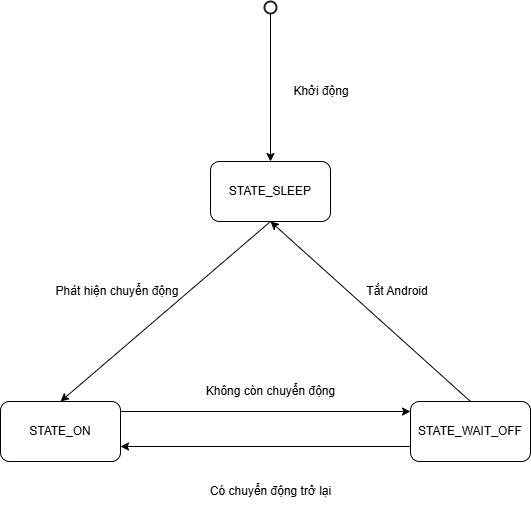
\includegraphics[width=0.8\textwidth]{Hinhve/State_machine.png}
    \caption{Sơ đồ mô hình máy trạng thái điều khiển hoạt động vi điều khiển ATmega8}
    \label{fig:state_machine}
\end{figure}

\end{document}
